\documentclass[11pt]{article}

\usepackage[a4paper,margin=1in]{geometry}
\usepackage{booktabs}
\usepackage{enumitem}
\usepackage{graphicx}
\usepackage{hyperref}
\usepackage{xcolor}

\hypersetup{
  colorlinks=true,
  linkcolor=blue!60!black,
  urlcolor=blue!60!black,
  citecolor=blue!60!black
}

\title{\textbf{Mega-Trading: Generative Order-Flow Modeling from Public Market Data}}
\author{Mega-Trading Project}
\date{Submitted take-home project}

\begin{document}
\maketitle

\begin{abstract}
Mega-Trading is a take-home prototype for modeling market-event sequences with
the same basic idea used by language models: predict the next token from recent
context. The project uses public Binance historical trade data, converts each
trade event into a discrete event token, trains a compact decoder-only
Transformer inspired by Llama-style language models, and evaluates the model on
a chronological holdout set. The design is motivated by recent work on
financial-market foundation models such as TradeFM, but this implementation is
intentionally smaller, reproducible, and based only on public data
\cite{binancepublic,tradefm,llama3,bommasani2021foundation}.
\end{abstract}

\section{System Overview}

The goal is to make the project easy to inspect. Public trade data is converted
into a sequence of simple event tokens. The model learns to predict the next
event token, and each generated token can be decoded back into market-event
features such as side, relative price depth, size bucket, and elapsed time. This
keeps the prototype close to the ``next token prediction'' pattern used in LLMs
while staying interpretable for market data \cite{vaswani2017attention,llama3}.

\section{Take-Home Scope}

The interview prompt was intentionally open-ended: build a non-trivial system,
choose the problem, decide how far to take it, define success criteria, and make
the work reviewable through version control. I used that prompt to build an
end-to-end system for generative market-event modeling rather than a single
notebook or isolated model experiment.

\begin{itemize}[leftmargin=1.6em]
  \item \textbf{Problem choice}: model public market events as a token sequence,
  inspired by the way LLMs learn next-token prediction.
  \item \textbf{Data system}: download public Binance trade data, normalize it
  into event fields, fit a tokenizer, and create chronological train,
  validation, and backtest splits.
  \item \textbf{Model and training system}: implement a decoder-only
  Transformer, train it with mixed precision, track metrics with MLflow, and
  optimize throughput with preloaded NumPy streams, \texttt{torch.compile}, and
  a Triton attention path.
  \item \textbf{Evaluation}: report held-out loss, perplexity, top-k accuracy,
  simple baselines, and generated vs. real event statistics.
  \item \textbf{System delivery}: package the checkpoint context, tokenizer
  metadata, reports, diagrams, and a Hugging Face Static Space page so the work
  can be reviewed end to end.
  \item \textbf{Version control}: keep configs, source modules, tests, and
  generated showcase artifacts separated so each part of the system is
  reviewable as a focused diff.
\end{itemize}

\section{Motivation and Fit}

I chose this project because it connects the company's market-data focus with my
own background as a research engineer building end-to-end foundation-model
systems. Deeter Analytics describes its mission as turning complex market data
into actionable insight with clarity, precision, foresight, and transparent
methodology \cite{deeteranalytics}. A generative market-event modeling system is
a natural take-home problem under that context: it starts from raw market data,
builds a model-visible representation, trains a sequence model, evaluates
outputs against held-out data, and packages the evidence for review.

My current work is on Amazon Nova foundation models, where the research
engineering role is to partner with researchers and help move model ideas from
experiments into production systems. Mega-Trading reflects that same operating
style at take-home scale: define a research-shaped problem, build the data and
training pipeline around it, optimize the system enough to run real experiments,
and present success criteria and limitations honestly.

\begin{figure}[t]
  \centering
  \fbox{\begin{minipage}{0.96\linewidth}
  \centering
  \textbf{Architecture figure:} \texttt{pipeline-figure.svg}\\[0.35em]
  The static Space renders the complete architecture figure from this SVG. For
  a PDF-only submission, export the SVG to PDF and replace this box with a
  standard \texttt{includegraphics} call.
  \end{minipage}}
  \caption{Mega-Trading data-to-model-to-output pipeline. The figure separates
  the data plane, tokenization, model core, training and evaluation, and
  inference output layers.}
  \label{fig:pipeline}
\end{figure}

\section{Data and Event Representation}

The data source is Binance's public historical trade archive, which can be
downloaded without private exchange credentials \cite{binancepublic}. Each raw
trade is mapped into a compact event representation:

\begin{itemize}[leftmargin=1.6em]
  \item \texttt{action}: simplified event type used by the model.
  \item \texttt{side}: buyer- or seller-initiated trade direction.
  \item \texttt{relative\_price\_bps}: log order price relative to estimated
  midprice.
  \item \texttt{price\_depth\_bps}: absolute relative price depth.
  \item \texttt{size}: causally normalized relative size.
  \item \texttt{interarrival\_seconds}: elapsed time since the prior event for
  the ticker.
\end{itemize}

The submitted dataset artifacts contain 62,012,828 token windows across 32
USDT symbols and 1,096 symbol-month partitions from 2023-05 to 2026-04. The
chronological split contains 54,695,345 train windows, 1,116,216 validation
windows, and 6,201,267 backtest windows.

\section{Tokenization}

The tokenizer turns each event into one integer ID. In plain terms, this is the
market-data analogue of turning a word into a token ID in an LLM. The ID is
formed from:
\[
  \texttt{action} \times \texttt{side} \times
  \texttt{relative\_price\_bucket} \times
  \texttt{price\_depth\_bucket} \times
  \texttt{size\_bucket} \times
  \texttt{time\_bucket}.
\]

The submitted tokenizer uses quantile binning with a 0.01 clip quantile. The
fitted vocabulary has 579 IDs, including special tokens. Realized bucket counts
are action=2, side=2, relative\_price=2, price\_depth=3, size=8, and time=3. This
choice keeps decoding auditable: every generated token maps back to an
event-feature tuple rather than an opaque vector.

\section{Model Architecture}

\texttt{TradingModel} is a decoder-only Transformer: it reads a context window
of prior event tokens and predicts the next event token. The implementation uses
standard modern LLM components, including token embeddings, RoPE positional
encoding, pre-norm decoder blocks, RMSNorm, grouped-query causal attention,
SwiGLU feed-forward layers, tied output embeddings, and a next-token cross
entropy objective \cite{vaswani2017attention,llama3}.

The submitted single-GPU model uses hidden size 1024, 20 decoder layers, 16
query heads, 4 key-value heads, feed-forward width 2816, context length 512, and
dropout 0. With the fitted vocabulary, this is approximately 226.1M
tied-embedding trainable parameters. The size was chosen to be large enough to
exercise a real Transformer training pipeline, but small enough to train and
debug on one high-memory CUDA GPU. Grouped-query attention lowers key-value
projection cost, RoPE handles causal sequence position without learned absolute
position tables, and tied embeddings reduce parameters while preserving a
simple token-language-model interface.

\section{Training and Optimization}

Training is orchestrated through Hydra and Hugging Face Accelerate. The
submitted run uses a hybrid optimizer setup: AdamW for embeddings and related
parameters, and Muon for large matrix parameters. It uses learning rate 0.0002
with cosine decay, 125 warmup steps, minimum learning rate \(2\times10^{-5}\),
batch size 64, mixed precision, Triton attention where available, and
\texttt{torch.compile} \cite{triton}.

Long single-GPU runs use prepared NumPy streams, persistent dataloader workers,
pinned host transfer, non-blocking device transfer, and a Triton attention path
where available.
The final submitted metric row reports 108K tokens/sec and a last-50-point mean
of 111K tokens/sec. MLflow is enabled; the tracking database contains 9 runs,
596,177 metric rows, 273 params, and 72 tags.

\section{Engineering Design Evidence}

The repository contains design and profiling notes that should be read as part
of the project evidence. They document decisions that are hard to infer from a
single final metric table:

\begin{itemize}
    \item \href{https://github.com/duoan/mega-trading/blob/main/docs/data-plane-design.md}{\texttt{docs/data-plane-design.md}} defines the Binance public-trades
    ingestion path, bounded-memory streaming prepare, tokenizer artifacts, and
    chronological split contract. This is the lineage layer behind every
    reported training and backtest metric.
    \item \href{https://github.com/duoan/mega-trading/blob/main/docs/training-plane-design.md}{\texttt{docs/training-plane-design.md}} records the NumPy shard input
    contract, checkpoint and manifest outputs, Accelerate-based DDP/FSDP
    execution path, and backtest handoff.
    \item \href{https://github.com/duoan/mega-trading/blob/main/docs/kernels.md}{\texttt{docs/kernels.md}} documents the Triton causal GQA attention
    path. On the submitted RTX-shape bf16 benchmark, the forward kernel reports
    156.23 approximate TFLOP/s versus 148.49 for PyTorch SDPA. The same note
    also records the current backward bottleneck: dK/dV register pressure and
    spills, so the limitation is explicit rather than hidden.
    \item \href{https://github.com/duoan/mega-trading/blob/main/docs/performance-profiling.md}{\texttt{docs/performance-profiling.md}} records the end-to-end PyTorch
    profiler investigation. The baseline CPU optimizer window was 323.645 ms
    over two optimizer updates; after the shape-bucketed Muon optimization with
    \texttt{training.muon\_ns\_steps=3}, it dropped to about 20.018 ms.
    \item \href{https://github.com/duoan/mega-trading/blob/main/docs/training-configs.md}{\texttt{docs/training-configs.md}} explains the Mac, RTX, Modal, and
    default environments. The same pipeline can run a smoke test, single-server
    CUDA training, or Modal GPU training through config-driven entry points.
    \item \href{https://github.com/duoan/mega-trading/blob/main/docs/training-systems-alignment.md}{\texttt{docs/training-systems-alignment.md}} maps the implementation
    to training-system concerns: throughput, GPU utilization, memory pressure,
    I/O bottlenecks, checkpoint reliability, failure recovery, and learning per
    unit of compute.
\end{itemize}

\section{Ablation Study}

\subsection*{Hypotheses}

The first ablation pass tested three practical hypotheses:

\begin{itemize}[leftmargin=1.6em]
  \item \textbf{Model capacity}: a small decoder should outperform a micro
  decoder on the same one-ticker slice.
  \item \textbf{Data size}: adding a second ticker should make the task harder
  at the same short training budget.
  \item \textbf{Training budget}: more steps should improve likelihood, but may
  not automatically improve generated rollout statistics.
\end{itemize}

The probe used Binance monthly trades for BTCUSDT and ETHUSDT in April 2026,
\texttt{block\_size=128}, \texttt{stride=4096}, 16 backtest batches, and 5
decoded examples per run. The goal was to validate the ablation workflow and
identify which dimensions are worth scaling next, not to claim a final
leaderboard.

\begin{table}[h]
  \centering
  \caption{Ablation probe results from \href{https://github.com/duoan/mega-trading/blob/main/docs/ablation-results.md}{\texttt{docs/ablation-results.md}}.}
  \begin{tabular}{llrrrrrr}
    \toprule
    Data & Model & Steps & Train & Val & Backtest & Top-1 & L1 \\
    \midrule
    1 ticker & micro & 20 & 3.410 & 2.915 & 3.060 & 0.619 & 0.632 \\
    1 ticker & small & 20 & 2.580 & 1.922 & 2.114 & 0.621 & 0.146 \\
    2 tickers & micro & 20 & 3.675 & 4.773 & 4.771 & 0.304 & 1.229 \\
    2 tickers & small & 20 & 2.797 & 4.990 & 4.943 & 0.004 & 0.141 \\
    2 tickers & small & 100 & 1.457 & 4.152 & 4.166 & 0.051 & 0.801 \\
    \bottomrule
  \end{tabular}
\end{table}

\begin{figure}[h]
  \centering
  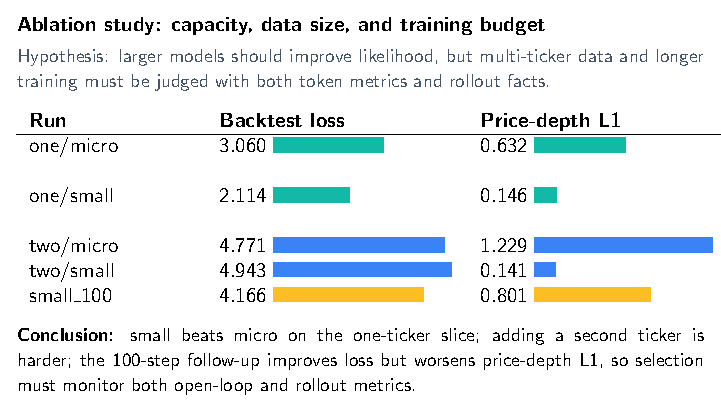
\includegraphics[width=\linewidth]{ablation-figure.pdf}
  \caption{Ablation study summary across backtest loss, price-depth L1, and
  top-1 accuracy. The result shows why model selection should monitor both
  open-loop token metrics and rollout stylized facts.}
\end{figure}

The cleanest conclusion is the one-ticker capacity result: moving from micro to
small reduced validation loss from 2.915 to 1.922, backtest loss from 3.060 to
2.114, and price-depth L1 from 0.632 to 0.146. The data-size result is more
subtle: adding ETHUSDT made next-token classification much harder at 20 steps,
even when the small model preserved a plausible marginal price-depth
distribution. The 100-step follow-up improved backtest loss from 4.943 to 4.166,
but worsened price-depth L1 from 0.141 to 0.801. The practical selection rule is
therefore to gate future runs on both likelihood and rollout realism.

\section{Backtest Results}

The submitted checkpoint was scored on 128 backtest batches, or 524,288 tokens.

\begin{table}[h]
  \centering
  \caption{Open-loop chronological backtest metrics.}
  \begin{tabular}{lr}
    \toprule
    Metric & Value \\
    \midrule
    Backtest loss & 2.3379 \\
    Backtest perplexity & 10.3592 \\
    Backtest top-1 accuracy & 49.23\% \\
    Backtest top-5 accuracy & 69.42\% \\
    Price-depth distribution L1 & 0.1420 \\
    \bottomrule
  \end{tabular}
\end{table}

Generated-versus-real stylized facts show that the model captures part of the
held-out event distribution but still mismatches tail behavior. Real excess
kurtosis is 3.0948; generated excess kurtosis is 14.2966. That gap is a concrete
target for better data, sampling, conditioning, and evaluation.

\section{Accuracy Baselines}

Top-1 accuracy should not be read against a vague random-guess baseline. With
579 realized token IDs, uniform random top-1 is only 0.17\% and uniform random
top-5 is 0.86\%. The more serious issue is token imbalance: on the exact
524,288-token scored backtest sample, only 135 labels appear and the effective
vocabulary is about 19.56.

\begin{table}[h]
  \centering
  \caption{Prediction baselines on the same scored backtest sample.}
  \begin{tabular}{lr}
    \toprule
    Baseline & Top-1 / coverage \\
    \midrule
    Uniform random top-1 & 0.17\% \\
    Uniform random top-5 & 0.86\% \\
    Cheating backtest majority token & 25.41\% \\
    Cheating backtest top-5 frequency coverage & 59.83\% \\
    Copy previous token & 33.63\% \\
    Train-sample unigram top-1 & 2.10\% \\
    Train-sample unigram top-5 & 8.27\% \\
    Train-sample one-step Markov argmax & 31.91\% \\
    Model top-1 & 49.23\% \\
    Model top-5 & 69.42\% \\
    \bottomrule
  \end{tabular}
\end{table}

The model is not worse than random and is meaningfully above copy-previous and
one-step Markov baselines. However, the metric is still not sufficient evidence
of trading usefulness because composite-token prediction is distribution-skewed.
Top-k accuracy should be treated as a sanity metric.

\section{Inference}

Inference uses the same files produced during training:

\begin{enumerate}[leftmargin=1.6em]
  \item Load \texttt{runs/rtx/checkpoint.pt}.
  \item Load \texttt{datasets/mixture=rtx/tokenizer.json} and
  \texttt{tokens-profile.json}.
  \item Validate the vocabulary size and context length.
  \item Provide either a recent context window or a beginning-of-sequence seed.
  \item Call \texttt{TradingModel.generate(input\_ids, max\_new\_tokens,
  top\_k=16)}.
  \item Decode generated token IDs back into event-feature tuples.
  \item Use decoded price-depth and side features for scenario charts or
  downstream simulation.
\end{enumerate}

This makes inference reproducible and auditable: every generated scenario can
be traced back through tokenizer metadata and model manifest fields.

\section{Limitations and Roadmap}

This is an open-loop public-data prototype. The current evaluation reports
chronological backtest loss, perplexity, top-k token accuracy, and
rollout-versus-real stylized facts. It does not yet implement the closed-loop
market simulator emphasized by TradeFM, which would validate order matching,
fills, queue dynamics, market impact, stress behavior, or execution-policy
performance \cite{tradefm}. The public Binance trade adapter is also only a
proxy for participant-observable order flow. Real L3 data should replace this
path for serious microstructure modeling.

Future directions are:

\begin{itemize}[leftmargin=1.6em]
  \item \textbf{L3 data}: ingest full add/delete/modify order lifecycle events,
  true best bid/ask midprice, queue position, and venue-specific order state.
  \item \textbf{Multimodal conditioning}: align news, filings, macro events,
  funding data, on-chain or flow signals, and sentiment with event-time
  order-flow tokens.
  \item \textbf{Closed-loop simulator}: evaluate generated events inside a
  deterministic LOB simulator to measure fills, slippage, spread dynamics, and
  market impact.
  \item \textbf{Inference packaging}: ship checkpoint, tokenizer, manifest, and
  model card together so generated scenarios preserve provenance.
  \item \textbf{Evaluation expansion}: add regime-conditioned metrics,
  tail-risk tests, execution-policy benchmarks, and calibration checks.
\end{itemize}

\begin{thebibliography}{9}

\bibitem{deeteranalytics}
Deeter Analytics Inc.
\newblock Company website.
\newblock \url{https://deeteranalytics.com/}.

\bibitem{binancepublic}
Binance.
\newblock Binance Public Data.
\newblock \url{https://data.binance.vision/}.

\bibitem{tradefm}
TradeFM.
\newblock \emph{TradeFM: A Generative Foundation Model for Trade-flow and
Market Microstructure}.
\newblock arXiv:2602.23784, 2026.

\bibitem{bommasani2021foundation}
Rishi Bommasani et al.
\newblock \emph{On the Opportunities and Risks of Foundation Models}.
\newblock arXiv:2108.07258, 2021.

\bibitem{vaswani2017attention}
Ashish Vaswani et al.
\newblock \emph{Attention Is All You Need}.
\newblock Advances in Neural Information Processing Systems, 2017.

\bibitem{llama3}
AI at Meta, Llama Team.
\newblock \emph{The Llama 3 Herd of Models}.
\newblock arXiv:2407.21783, 2024.

\bibitem{triton}
Philippe Tillet, H. T. Kung, and David Cox.
\newblock \emph{Triton: An Intermediate Language and Compiler for Tiled Neural
Network Computations}.
\newblock MAPL, 2019. \url{https://doi.org/10.1145/3315508.3329973}.

\end{thebibliography}

\end{document}
